\begin{frame}
	\frametitle{Dise\~no}
	\framesubtitle{SOLID y patrones}
	\begin{columns}[T]
		
		\begin{column}[T]{0.5\linewidth}
			\begin{block}{SOLID}
				\begin{itemize}
					\item \textbf{S}ingle responsibility principle
					\item \textbf{O}pen-closed principle
					\item \textbf{L}iskov substitution principle
					\item \textbf{I}nterface segregation principle
					\item \textbf{D}ependency inversion principle
				\end{itemize}
			\end{block}
		\end{column}
		
		\begin{column}[T]{0.5\linewidth}
			\begin{block}{Patrones}
				\begin{itemize}
					\item Model View View-Model
					\item Iterator
					\item Singleton
				\end{itemize}
			\end{block}
		\end{column}
		
	\end{columns}

\end{frame}

%\section{Desarrollo}
\begin{frame}
	\frametitle{Desarrollo}
	\framesubtitle{Qu\'e se ha hecho}
	Una aplicaci\'on que permite:
	\begin{enumerate}
		\item Cargar un XML con las observaciones y propiedades
		\item Visualizar datos discretos y continuos
		\item Cargar v\'ideos y visualizarlos
		\item Seleccionar rangos
		\item Exportar los rangos seleccionados en XML
		\item Interfaz tipo IDE, como Eclipse o Visual 
		Studio
	\end{enumerate}
	
\end{frame}

\begin{frame}
    \frametitle{Desarrollo}
    \framesubtitle{C\'omo se ha hecho}
    \begin{block}{Cargar un XML con las observaciones y propiedades}
        
        \begin{itemize}
            \item Se ha utilizado LINQ to XML
            \item Permite realizar consultas similares a SQL a los XML
        \end{itemize}
        
    \end{block}
    
\end{frame}

\begin{frame}[fragile]
    \frametitle{Desarrollo}
    \framesubtitle{C\'omo se ha hecho}
    
    \begin{block}{Ejemplo LINQ To XML}
        \begin{lstlisting}[ breaklines=true, language=C, 
        numbers=left, 
        showspaces=false]
        private IEnumerable<XElement> getData(string observacion)
        {
            return from prop in xml.Descendants("property")
                where (string)prop.Parent.Attribute("name") == 
                observacion
                select prop;
        }
        \end{lstlisting}
    \end{block}
\end{frame}

\begin{frame}
    \frametitle{Desarrollo}
    \framesubtitle{C\'omo se ha hecho}
    
    \begin{block}{Seleccionar rangos}
        
        \begin{columns}[T]
            \begin{column}[T]{0.5\linewidth}
                \begin{enumerate}
                    \item Cada propiedad notifica a su padre cuando cambia
                    \item Esa observaci\'on notifica al Gestor de gr\'aficos 
                    \item El gestor cicla a trav\'es de todas las observaciones
                    \item Cada observaci\'on actualiza el valor de sus 
                    propiedades
                \end{enumerate}
            \end{column}
            
            \begin{column}[T]{0.5\linewidth}
                    
                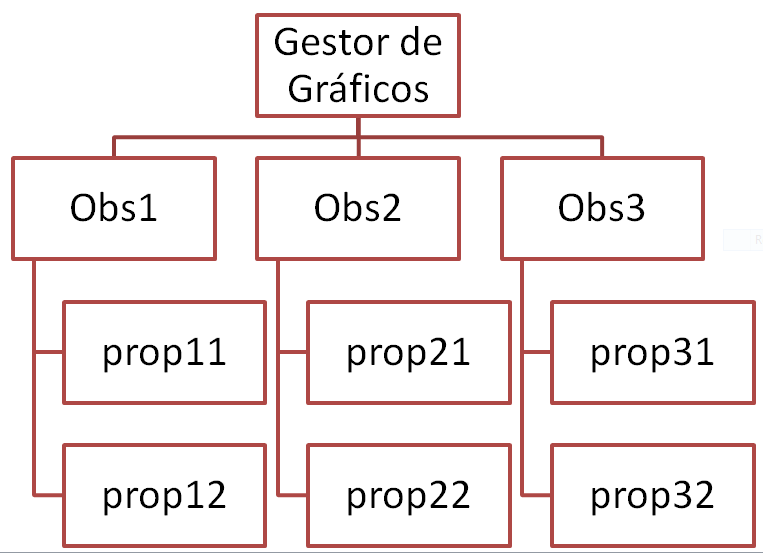
\includegraphics[width=1.0\linewidth]{Figures/EstructuraDatos.PNG}
               
            \end{column}
        \end{columns}
       
    \end{block}
\end{frame}

\begin{frame}
    \frametitle{Desarrollo}
    \framesubtitle{C\'omo se ha hecho}
    
    \begin{block}{Exportar los rangos seleccionados}
        
        \begin{itemize}
            \item Igual que cargar, pero al rev\'es
            \item Se usa LINQ para obtener los datos de los View-Models
            \item Se crean los elementos XML y se van guardando
            \item Finalmente se exportan haciendo \emph{.toString()}
        \end{itemize}
        
    \end{block}
\end{frame}

\begin{frame}
    \frametitle{Desarrollo}
    \framesubtitle{C\'omo se ha hecho}
    
    \begin{block}{Interfaz tipo IDE}
        \begin{figure}
            \centering
            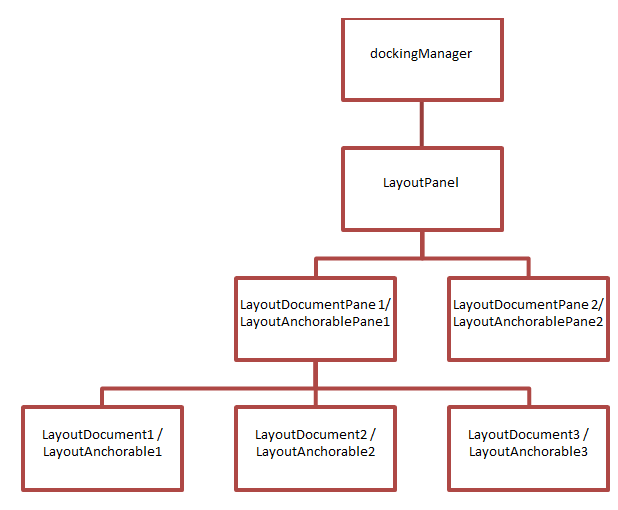
\includegraphics[width=0.6\linewidth]{Figures/AvalonDock.PNG}
        \end{figure}
        

    \end{block}
\end{frame}

%\section{Herramientas utilizadas}
\begin{frame}
	\frametitle{Desarrollo}
	\framesubtitle{Herramientas utilizadas}
	
	\begin{itemize}
		\item Visual Studio 2013 Ultimate
		\item OxyPlot
		\item AvalonDock
		\item Git
		\item \LaTeX y TeXstudio
	\end{itemize}
\end{frame}